\documentclass[a4paper, twocolumn, landscape, 9pt]{article}
\usepackage[utf8]{inputenc}
\usepackage[T1]{fontenc}
\usepackage{multicol}
\usepackage[margin=0.5in, bmargin=0.4in, tmargin=0.8in]{geometry}
\usepackage{titlesec}
\usepackage{etoolbox}
\usepackage{fancyhdr}
\usepackage[titles]{tocloft}
\usepackage{graphicx}
\usepackage{listings}
\usepackage{amsmath}
\usepackage{hyperref}

\hypersetup{
  colorlinks,
  citecolor=black,
  filecolor=black,
  linkcolor=black,
  urlcolor=black
}

\pagestyle{fancy}
\fancyhf{}
\rhead{Page \thepage}
\lhead{Federal University of Bahia - Universidade Federal da Bahia}

\lstset{
language=R,
literate=
{≡}{{$\equiv$}}1
{∩}{{$\cap$}}1
{∪}{{$\cup$}}1
{∛N}{{$\sqrt[3]{N}$}}1
{Ã}{{\~A}}1
{Á}{{\'A}}1
{Â}{{\^A}}1
{á}{{\'a}}1
{à}{{\`a}}1
{ã}{{\~a}}1
{â}{{\^a}}1
{é}{{\'e}}1
{É}{{\'E}}1
{ê}{{\^e}}1
{í}{{\'i}}1
{ó}{{\'o}}1
{ô}{{\^o}}1
{õ}{{\~o}}1
{ú}{{\'u}}1
{ü}{{\"u}}1
{ç}{{\c{c}}}1
}

\usepackage{xcolor}
\usepackage{listings}
% \usepackage{courier}
\usepackage{courier}
\usepackage{pgfplotstable}
% recommended:
\usepackage{booktabs}
\usepackage{array}
\usepackage{colortbl}
\usepackage{verbatim}
\usepackage{xstring}

\definecolor{mygreen}{rgb}{0,0.6,0}
\definecolor{mygray}{rgb}{0.5,0.5,0.5}
\definecolor{mymauve}{rgb}{0.58,0,0.82}
\definecolor{codegreen}{rgb}{0,0.6,0}
\definecolor{codegray}{rgb}{0.5,0.5,0.5}
\definecolor{codepurple}{rgb}{0.58,0,0.82}
\definecolor{backcolour}{rgb}{0.95,0.95,0.92}

\def\trim#1{\ignorespaces#1\unskip} 

\lstset{ %
  basicstyle=\linespread{0.82}\footnotesize\ttfamily,        % the size of the fonts that are used for the code
  breakatwhitespace=true,         % sets if automatic breaks should only happen at whitespace
  breaklines=true,                 % sets automatic line breaking
  commentstyle=\itshape\color{black!63},    % comment style
  extendedchars=true,              % lets you use non-ASCII characters; for 8-bits encodings only, does not work with UTF-8
  frame=lbtr,                    % adds a frame around the code
  keepspaces=true,                 % keeps spaces in text, useful for keeping indentation of code (possibly needs columns=flexible)
  keywordstyle=\bfseries,       % keyword style
  numbers=left,                    % where to put the line-numbers; possible values are (none, left, right)
  numbersep=8pt,                   % how far the line-numbers are from the code
  numberstyle=\scriptsize, % the style that is used for the line-numbers
  rulecolor=\color{black},         % if not set, the frame-color may be changed on line-breaks within not-black text (e.g. comments (green here))
  showspaces=false,                % show spaces everywhere adding particular underscores; it overrides 'showstringspaces'
  showstringspaces=false,          % underline spaces within strings only
  showtabs=false,                  % show tabs within strings adding particular underscores
  stringstyle=,     % string literal style
  tabsize=2,                     % sets default tabsize to 2 spaces
  inputencoding=utf8
}

\lstdefinestyle{colored}{
  basicstyle=\footnotesize\ttfamily,
  keywordstyle=\color{green!30!black},
  commentstyle=\itshape\color{purple!40!black},
  identifierstyle=,
  stringstyle=\color{orange},
}

\lstdefinestyle{mystyle}{
  %backgroundcolor=\color{backcolour},   
  commentstyle=\color{green!30!black},
  keywordstyle=\color{magenta},
  numberstyle=\color{codegray},
  stringstyle=\color{codepurple},
  rulecolor=\color{codegray},
}

\lstset{columns=fullflexible}

\def\EOF{1000}

\def\normLineNumber#1{\trim{\detokenize{#1}}}

\newcommand{\includenote}[1]{\lstinputlisting{codes/#1}}
\newcommand{\includecode}[2][C++]{
  \lstinputlisting[escapechar=, language=#1]{codes/#2}
}

\newcommand{\includepiece}[3][C++]{
  %{\detokenize{#2} (\normLineNumber{#3})}
  \lstinputlisting[escapechar=, language=#1, linerange={#3}]{codes/#2}
}

% \pgfplotstabletypeset{col sep=tab}

\newcommand{\includetable}[1]{
  \begin{verbatim}\input{notes/#1}\end{verbatim}
}


% usage of commands
% section, subsection and subsubsection were renewed so they receive 2 arguments instead of 1. ex: \section{title}{text}
% \includecode[language]{file} include code from codes/{file}. default language is C++.
% \includepiece[language]{file}{firstline}{lastline} does the same thing, but it includes from firstline to lastline only.
%

%% Control the fonts and formatting used in the table of contents.

%% Aesthetic spacing redefines that look nicer to me than the defaults.

\setlength{\cftbeforesecskip}{0.02em}
\setlength{\cftbeforesubsecskip}{0.02em}
\setlength{\cftbeforesubsubsecskip}{0.02em}

%% Use Helvetica-Narrow Bold for Chapter entries

\renewcommand{\cftsecfont}{%
  \fontsize{10}{10}\usefont{T1}{phv}{bc}{n}\selectfont
}
\renewcommand{\cftsubsecfont}{
  \fontsize{9}{9}\usefont{T1}{phv}{c}{n}\selectfont
}
\renewcommand{\cftsubsubsecfont}{
  \fontsize{9}{9}\usefont{T1}{phv}{c}{n}\selectfont
}


\renewcommand{\familydefault}{\ttdefault}
\setlength{\columnsep}{1cm}

\let\Asection\section
\let\Bsection\subsection
\let\Csection\subsubsection

\renewcommand{\section}[2]{
  \ifstrequal{#2}{}{\Asection[#1 *]{#1} #2}{\Asection{#1} #2} %
}
\renewcommand{\subsection}[2]{
  \ifstrequal{#2}{}{\Bsection[#1 *]{#1} #2}{\Bsection{#1} #2} %
}
\renewcommand{\subsubsection}[2]{
  \ifstrequal{#2}{}{\Csection[#1 *]{#1} #2}{\Csection{#1} #2} %
}

\title{C++ Competitive Programming Library \\ \large ***DO NOT DISCLOSE OR DISTRIBUTE***}
\author{bfs.07 - Bernardo Flores Salmeron}
\date{}

\begin{document}

\titleformat{\section}[hang]{\large}{}{0pt}{\thesection. }
\titleformat{\subsection}[hang]{\normalsize}{}{0pt}{\thesubsection. }
\titleformat{\subsubsection}[hang]{\small}{}{0pt}{\thesubsubsection. }
\titlespacing{\section}{0px}{3px}{2px}
\titlespacing{\subsection}{0px}{2px}{1px}

% generate title and table of contents with no heading
\maketitle
\thispagestyle{fancy}

\makeatletter
%\renewcommand{\l@subsection}{\@dottedtocline{2}{1.5em}{3.0em}}
%\renewcommand{\l@subsubsection}{\@dottedtocline{3}{3.0em}{4em}}
\def\tableofcontents{\@starttoc{toc}}
\makeatother

%\centering\textcolor{red}{\textbf{THE WHOLE LIB USES dcmp() FOR FLOATING-POINT COMPARISON}}

\tableofcontents

\newpage

\section{Template}{
  \includecode{"template.cpp"}
}

\section{Data Structures}{

  \subsection{Bit2D}{
    \includecode{"data_structures/BIT2D.cpp"}
  }

  \subsection{Merge Sort Tree (K-Esimo Maior Elemento Num Intervalo, Valores Maiores Que K Num Intervalo, }{
    \includecode{"data_structures/Merge Sort Tree (K-ESIMO MAIOR ELEMENTO NUM INTERVALO, VALORES MAIORES QUE K NUM INTERVALO, ...).cpp"}
  }

  \subsection{Mos Algorithm}{
    \includecode{"data_structures/Mos Algorithm.cpp (Most frequent Value in intervals).cpp"}
  }

  \subsection{Ordenacao De Estruturas (Pq, Etc)}{
    \includecode{"data_structures/Ordenacao de Estruturas (PQ, etc).cpp"}
  }

  \subsection{Sqrt Decomposition}{
    \includecode{"data_structures/SQRT Decomposition.cpp"}
  }

  \subsection{Bit}{
    \includecode{"data_structures/bit.cpp"}
  }

  \subsection{Bit (Range Update)}{
    \includecode{"data_structures/bit_(range_update).cpp"}
  }

  \subsection{Counting Inversions (Minimum Number Of Adjacent Swaps To Sort Array)}{
    \includecode{"data_structures/counting_inversions_(minimum_number_of_adjacent_swaps_to_sort_array).cpp"}
  }

  \subsection{Ordered Set}{
    \includecode{"data_structures/ordered_set.cpp"}
  }

  \subsection{Persistent Segment Tree}{
    \includecode{"data_structures/persistent_segment_tree.cpp"}
  }

  \subsection{Segment Tree}{
    \includecode{"data_structures/segment_tree.cpp"}
  }

  \subsection{Segment Tree 2D}{
    \includecode{"data_structures/segment_tree_2d.cpp"}
  }

  \subsection{Segment Tree Polynomial}{
    \includecode{"data_structures/segment_tree_polynomial.cpp"}
  }

  \subsection{Sparse Table}{
    \includecode{"data_structures/sparse_table.cpp"}
  }

}

\section{Dp}{

  \subsection{Achar Maior Palindromo}{
    \includecode{"dp/Achar Maior Palindromo.txt"}
  }

  \subsection{Digit Dp}{
    \includecode{"dp/Digit DP.cpp"}
  }

  \subsection{Longest Common Subsequence}{
    \includecode{"dp/Longest Common Subsequence.cpp"}
  }

  \subsection{Longest Common Substring}{
    \includecode{"dp/Longest Common Substring.cpp"}
  }

  \subsection{Longest Increasing Subsequence 2D (Not Sorted)}{
    \includecode{"dp/Longest Increasing Subsequence 2D (not sorted).cpp"}
  }

  \subsection{Longest Increasing Subsequence 2D (Sorted)}{
    \includecode{"dp/Longest Increasing Subsequence 2D (sorted).cpp"}
  }

  \subsection{Longest Increasing Subsequence}{
    \includecode{"dp/Longest Increasing Subsequence.cpp"}
  }

  \subsection{Subset Sum Com Bitset}{
    \includecode{"dp/Subset Sum com Bitset.cpp"}
  }

  \subsection{Catalan}{
    \begin{figure}[h!]
      \centering
      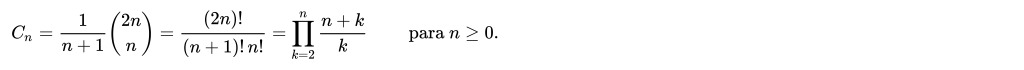
\includegraphics[scale=0.7]{"codes/dp/catalan.jpg"}
    \end{figure}
  }

  \subsection{Catalan }{
    \includecode{"dp/catalan_.cpp"}
  }

  \subsection{Coin Change Problem}{
    \includecode{"dp/coin_change_problem.cpp"}
  }

  \subsection{Knapsack}{
    \includecode{"dp/knapsack.cpp"}
  }

}

\section{Geometry}{

  \subsection{Centro De Massa De Um Poligono}{
    \includecode{"geometry/Centro de Massa de um Poligono.cpp"}
  }

  \subsection{Closest Pair Of Points}{
    \includecode{"geometry/Closest Pair of Points.cpp"}
  }

  \subsection{Condicao De Existencia De Um Triangulo}{
    \includecode{"geometry/Condicao de Existencia de um Triangulo.txt"}
  }

  \subsection{Convex Hull}{
    \includecode{"geometry/Convex Hull.cpp"}
  }

  \subsection{Cross Product}{
    \includecode{"geometry/Cross Product.cpp"}
  }

  \subsection{Distance Point Segment}{
    \includecode{"geometry/Distance Point Segment.cpp"}
  }

  \subsection{Line-Line Intersection}{
    \includecode{"geometry/Line-Line Intersection.cpp"}
  }

  \subsection{Line-Point Distance}{
    \includecode{"geometry/Line-Point Distance.cpp"}
  }

  \subsection{Point Inside Convex Polygon - Log(N)}{
    \includecode{"geometry/Point Inside Convex Polygon - log(n).cpp"}
  }

  \subsection{Point Inside Polygon}{
    \includecode{"geometry/Point Inside Polygon.cpp"}
  }

  \subsection{Points Inside And In Boundary Polygon}{
    \includecode{"geometry/Points Inside and in Boundary Polygon.cpp"}
  }

  \subsection{Polygon Area (3D)}{
    \includecode{"geometry/Polygon Area (3d).cpp"}
  }

  \subsection{Polygon Area}{
    \includecode{"geometry/Polygon Area.cpp"}
  }

  \subsection{Segment-Segment Intersection}{
    \includecode{"geometry/Segment-Segment Intersection.cpp"}
  }

  \subsection{Upper And Lower Hull}{
    \includecode{"geometry/Upper and Lower Hull.cpp"}
  }

  \subsection{Circle Circle Intersection}{
    \begin{figure}[h!]
      \centering
      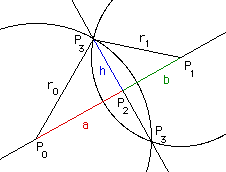
\includegraphics[scale=0.7]{"codes/geometry/circle_circle_intersection.jpg"}
    \end{figure}
  }

  \subsection{Circle Circle Intersection }{
    \includecode{"geometry/circle_circle_intersection_.cpp"}
  }

  \subsection{Struct Point And Line}{
    \includecode{"geometry/struct Point and Line.cpp"}
  }

}

\section{Graphs}{

  \subsection{Checa Grafo Bipartido}{
    \includecode{"graphs/Checa Grafo Bipartido.cpp"}
  }

  \subsection{Ciclo Grafo}{
    \includecode{"graphs/Ciclo Grafo.cpp"}
  }

  \subsection{Diametro Em Arvore}{
    \includecode{"graphs/Diametro em Arvore.txt"}
  }

  \subsection{Ford Fulkersson (Maximum Flow)}{
    \includecode{"graphs/Ford Fulkersson (Maximum Flow).cpp"}
  }

  \subsection{Pontes Num Grafo}{
    \includecode{"graphs/Pontes num Grafo.cpp"}
  }

  \subsection{Pontos De Articulacao}{
    \includecode{"graphs/Pontos de Articulacao.cpp"}
  }

  \subsection{Scc (Kosaraju)}{
    \includecode{"graphs/SCC_(Kosaraju).cpp"}
  }

  \subsection{All Eulerian Path Or Tour}{
    \includecode{"graphs/all_eulerian_path_or_tour.cpp"}
  }

  \subsection{Bellman Ford}{
    \includecode{"graphs/bellman_ford.cpp"}
  }

  \subsection{De Bruijn Sequence}{
    \includecode{"graphs/de_bruijn_sequence.cpp"}
  }

  \subsection{Dijkstra + Dij Graph}{
    \includecode{"graphs/dijkstra_+_dij_graph.cpp"}
  }

  \subsection{Dinic (Max Flow)}{
    \includecode{"graphs/dinic_(max_flow).cpp"}
  }

  \subsection{Floyd Warshall}{
    \includecode{"graphs/floyd_warshall.cpp"}
  }

  \subsection{Functional Graph}{
    \includecode{"graphs/functional_graph.cpp"}
  }

  \subsection{Hld}{
    \includecode{"graphs/hld.cpp"}
  }

  \subsection{Kruskal + Dsu}{
    \includecode{"graphs/kruskal_+_dsu.cpp"}
  }

  \subsection{Lca}{
    \includecode{"graphs/lca.cpp"}
  }

  \subsection{Maximum Path Unweighted Graph}{
    \includecode{"graphs/maximum_path_unweighted_graph.cpp"}
  }

  \subsection{Number Of Different Spanning Trees In A Complete Graph}{
    \includecode{"graphs/number_of_different_spanning_trees_in_a_complete_graph.txt"}
  }

  \subsection{Number Of Ways To Make A Graph Connected}{
    \includecode{"graphs/number_of_ways_to_make_a_graph_connected.txt"}
  }

  \subsection{Pruffer Decode}{
    \includecode{"graphs/pruffer_decode.cpp"}
  }

  \subsection{Pruffer Encode}{
    \includecode{"graphs/pruffer_encode.cpp"}
  }

  \subsection{Pruffer Properties}{
    \includecode{"graphs/pruffer_properties.txt"}
  }

  \subsection{Remove All Bridges From Graph}{
    \includecode{"graphs/remove_all_bridges_from_graph.txt"}
  }

  \subsection{Shortest Cycle In A Graph}{
    \includecode{"graphs/shortest_cycle_in_a_graph.cpp"}
  }

  \subsection{Topological Sort}{
    \includecode{"graphs/topological_sort.cpp"}
  }

  \subsection{Tree Distance}{
    \includecode{"graphs/tree_distance.cpp"}
  }

}

\section{Language Stuff}{

  \subsection{Binary String To Int}{
    \includecode{"language_stuff/Binary String to Int.cpp"}
  }

  \subsection{Climits}{
    \includecode{"language_stuff/CLIMITS.cpp"}
  }

  \subsection{Checagem Brute Force Com Solucao}{
    \includecode{"language_stuff/Checagem Brute Force com Solucao.cpp"}
  }

  \subsection{Checagem De Bits}{
    \includecode{"language_stuff/Checagem de Bits.cpp"}
  }

  \subsection{Checagem E Tranformacao De Caractere}{
    \includecode{"language_stuff/Checagem e Tranformacao de Caractere.cpp"}
  }

  \subsection{Conta Digitos 1 Ate N}{
    \includecode{"language_stuff/Conta Digitos 1 ate N.cpp"}
  }

  \subsection{Escrita Em Arquivo}{
    \includecode{"language_stuff/Escrita em Arquivo.cpp"}
  }

  \subsection{Gcd}{
    \includecode{"language_stuff/GCD.cpp"}
  }

  \subsection{Hipotenusa}{
    \includecode{"language_stuff/Hipotenusa.cpp"}
  }

  \subsection{Int To Binary String}{
    \includecode{"language_stuff/Int to Binary String.cpp"}
  }

  \subsection{Int To String}{
    \includecode{"language_stuff/Int to String.cpp"}
  }

  \subsection{Leitura De Arquivo}{
    \includecode{"language_stuff/Leitura de Arquivo.cpp"}
  }

  \subsection{Max E Min Element Num Vetor}{
    \includecode{"language_stuff/Max e Min Element num vetor.cpp"}
  }

  \subsection{Permutacao}{
    \includecode{"language_stuff/Permutacao.cpp"}
  }

  \subsection{Printf De Uma String}{
    \includecode{"language_stuff/Printf de uma string.cpp"}
  }

  \subsection{Remove Repeticoes Continuas Num Vetor}{
    \includecode{"language_stuff/Remove Repeticoes Continuas num Vetor.cpp"}
  }

  \subsection{Rotate (Left)}{
    \includecode{"language_stuff/Rotate (Left).cpp"}
  }

  \subsection{Rotate (Right)}{
    \includecode{"language_stuff/Rotate (Right).cpp"}
  }

  \subsection{Scanf De Uma String}{
    \includecode{"language_stuff/Scanf de uma string.cpp"}
  }

  \subsection{Split Function}{
    \includecode{"language_stuff/Split Function.cpp"}
  }

  \subsection{String To Long Long}{
    \includecode{"language_stuff/String to Long Long.cpp"}
  }

  \subsection{Substring}{
    \includecode{"language_stuff/Substring.cpp"}
  }

  \subsection{Width}{
    \includecode{"language_stuff/Width.cpp"}
  }

  \subsection{Check Overflow}{
    \includecode{"language_stuff/check_overflow.txt"}
  }

  \subsection{Readint}{
    \includecode{"language_stuff/readint.cpp"}
  }

}

\section{Math}{

  \subsection{Bell Numbers}{
    \includecode{"math/Bell Numbers.cpp"}
  }

  \subsection{Checagem De Primalidade}{
    \includecode{"math/Checagem de Primalidade.cpp"}
  }

  \subsection{Combinacao Ncr Mod Primo}{
    \includecode{"math/Combinacao nCr mod Primo.cpp"}
  }

  \subsection{Combinacao Ncr}{
    \includecode{"math/Combinacao nCr.cpp"}
  }

  \subsection{Compressao De Pontos}{
    \includecode{"math/Compressao de Pontos.cpp"}
  }

  \subsection{Equacao Diofantina}{
    \includecode{"math/Equacao Diofantina.cpp"}
  }

  \subsection{Euclides Estendido}{
    \includecode{"math/Euclides Estendido.cpp"}
  }

  \subsection{Euler Totient}{
    \includecode{"math/Euler Totient.cpp"}
  }

  \subsection{Fatoracao Multiplas Queries}{
    \includecode{"math/Fatoracao Multiplas Queries.cpp"}
  }

  \subsection{Fatoracao Simples}{
    \includecode{"math/Fatoracao Simples.cpp"}
  }

  \subsection{Numero De Fatores}{
    \includecode{"math/Numero de Fatores.cpp"}
  }

  \subsection{Pollard Rho (Find A Divisor)}{
    \includecode{"math/Pollard Rho (Find a Divisor).cpp"}
  }

  \subsection{Precomputar Combinacao Ncr}{
    \includecode{"math/Precomputar Combinacao nCr.cpp"}
  }

  \subsection{Teorema Chines Do Resto}{
    \includecode{"math/Teorema Chines do Resto.cpp"}
  }

  \subsection{Binary Exponentiation}{
    \includecode{"math/binary_exponentiation.cpp"}
  }

  \subsection{Combinatorics}{
    \includecode{"math/combinatorics.cpp"}
  }

  \subsection{Divisors}{
    \includecode{"math/divisors.cpp"}
  }

  \subsection{Inclusion Exclusion}{
    \begin{figure}[h!]
      \centering
      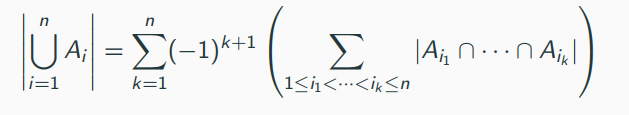
\includegraphics[scale=0.7]{"codes/math/inclusion_exclusion.jpg"}
    \end{figure}
  }

  \subsection{Inclusion Exclusion }{
    \includecode{"math/inclusion_exclusion_.cpp"}
  }

  \subsection{Matrix Exponentiation}{
    \includecode{"math/matrix_exponentiation.cpp"}
  }

  \subsection{Modular Inverse}{
    \includecode{"math/modular_inverse.cpp"}
  }

  \subsection{Sieve + Segmented Sieve}{
    \includecode{"math/sieve_+_segmented_sieve.cpp"}
  }

}

\section{Miscellaneous}{

  \subsection{2-Sat}{
    \includecode{"miscellaneous/2-SAT.cpp"}
  }

  \subsection{3Sum Problem}{
    \includecode{"miscellaneous/3SUM Problem.cpp"}
  }

  \subsection{Fibonacci Matrix Exponentiation}{
    \includecode{"miscellaneous/Fibonacci Matrix Exponentiation.cpp"}
  }

  \subsection{Infix To Prefix}{
    \includecode{"miscellaneous/Infix to Prefix.cpp"}
  }

  \subsection{Interval Scheduling}{
    \begin{figure}[h!]
      \centering
      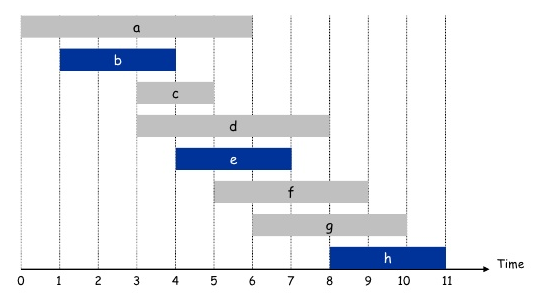
\includegraphics[scale=0.7]{"codes/miscellaneous/Interval Scheduling.jpg"}
    \end{figure}
  }

  \subsection{Interval Scheduling}{
    \includecode{"miscellaneous/Interval Scheduling.txt"}
  }

  \subsection{Kadane (Maior Soma Num Vetor)}{
    \includecode{"miscellaneous/Kadane (Maior soma num Vetor).cpp"}
  }

  \subsection{Kadane 2D}{
    \includecode{"miscellaneous/Kadane 2d.cpp"}
  }

  \subsection{Oito Rainhas}{
    \includecode{"miscellaneous/Oito Rainhas.cpp"}
  }

  \subsection{Sliding Window Minimum}{
    \includecode{"miscellaneous/Sliding Window Minimum.cpp"}
  }

  \subsection{Torre De Hanoi}{
    \includecode{"miscellaneous/Torre de Hanoi.cpp"}
  }

  \subsection{Kadane (Segment Tree)}{
    \includecode{"miscellaneous/kadane_(segment_tree).cpp"}
  }

  \subsection{Largest Area In Histogram}{
    \includecode{"miscellaneous/largest_area_in_histogram.cpp"}
  }

  \subsection{Point Compression}{
    \includecode{"miscellaneous/point_compression.cpp"}
  }

}

\section{Strings}{

  \subsection{Kmp}{
    \includecode{"strings/KMP.cpp"}
  }

  \subsection{Trie - Maximum Xor Sum}{
    \includecode{"strings/Trie - Maximum XOR Sum.txt"}
  }

  \subsection{Trie - Maximum Xor Two Elements}{
    \includecode{"strings/Trie - Maximum XOR two elements.txt"}
  }

  \subsection{Z-Function}{
    \includecode{"strings/Z-Function.cpp"}
  }

  \subsection{Aho Corasick}{
    \includecode{"strings/aho_corasick.cpp"}
  }

  \subsection{Hashing}{
    \includecode{"strings/hashing.cpp"}
  }

  \subsection{Lcs K Strings}{
    \includecode{"strings/lcs_k_strings.cpp"}
  }

  \subsection{Lexicographically Smallest Rotation}{
    \includecode{"strings/lexicographically_smallest_rotation.cpp"}
  }

  \subsection{Manacher (Longest Palindrome)}{
    \includecode{"strings/manacher_(longest_palindrome).cpp"}
  }

  \subsection{Suffix Array}{
    \includecode{"strings/suffix_array.cpp"}
  }

  \subsection{Suffix Array Pessoa}{
    \includecode{"strings/suffix_array_pessoa.cpp"}
  }

  \subsection{Suffix Array With Additional Memory}{
    \includecode{"strings/suffix_array_with_additional_memory.cpp"}
  }

  \subsection{Trie}{
    \includecode{"strings/trie.cpp"}
  }

}

\end{document}
